%----------------------------------------------------------------------------------------
%	PACKAGES AND THEMES
%----------------------------------------------------------------------------------------
\documentclass[aspectratio=169,xcolor=dvipsnames]{beamer}
\usetheme{Madrid}
\usecolortheme{beaver}

\usepackage{xcolor}
\definecolor{redcol}{RGB}{252, 33, 33}
\setbeamercolor{item}{fg=redcol}

\usepackage{hyperref}
\usepackage{graphicx} % Allows including images
\usepackage{booktabs} % Allows the use of \toprule, \midrule and \bottomrule in tables

%% The amssymb package provides various useful mathematical symbols
\usepackage{amsmath}
\usepackage{amssymb}
\usepackage{lipsum}
\usepackage{mathrsfs}
\usepackage{bm}
\usepackage{xcolor}

\usepackage{algorithm}
\usepackage{algpseudocode}

\usepackage{amsthm}

\usepackage{listings}
\lstset{language=Python}
\usepackage{inconsolata}
\lstset{
  basicstyle=\ttfamily\footnotesize, % font size and family
  columns=flexible, % better spacing
  keepspaces=true, % respects spaces
}

\newtheoremstyle{named}{}{}{\itshape}{}{\bfseries}{.}{.5em}{\thmnote{#3's }#1}
\theoremstyle{named}
\newtheorem*{namedtheorem}{Theorem}

\newtheorem{assumption}{Assumption}

\newcommand{\indep}{\perp \!\!\! \perp}
\newcommand{\modelg}{\mathbf{g}}

%----------------------------------------------------------------------------------------
%	TITLE PAGE
%----------------------------------------------------------------------------------------

% The title
\title[PBL Reading Club]{Diffusion Models}

\author[Dayta] {Dayta, Dominic Bagus}
\institute[NAIST] % Your institution may be shorthand to save space
{
    % Your institution for the title page
    Mathematical Informatics Laboratory \\
    Nara Institute of Science and Technology 
    \vskip 3pt
}
\date{31 July, 2025} % Date, can be changed to a custom date


%----------------------------------------------------------------------------------------
%	PRESENTATION SLIDES
%----------------------------------------------------------------------------------------

\begin{document}

\begin{frame}
    % Print the title page as the first slide
    \titlepage
\end{frame}

\begin{frame}{Overview}
    % Throughout your presentation, if you choose to use \section{} and \subsection{} commands, these will automatically be printed on this slide as an overview of your presentation
    \tableofcontents
\end{frame}

%------------------------------------------------
\section{Introduction}
%------------------------------------------------

\begin{frame}{Generative Models}

Previous sections have demonstrated the power of \alert{generative latent models}: we suppose the data space $\mathbf{x}$ arises from a latent space $\mathbf{z}$ with probability distribution $p(\mathbf{z})$.

\vspace{0.5cm}

\alert{Diffusion models}, also called \textit{denoising diffusion probabilistic models}, or DDPMs follows this same idea.

\vspace{0.5cm}

We take each training image $x_i$ and to corrupt it using a multi-step noise process to transform it into a Gaussian sample $z_i$. A deep neural network is then trained to invert this process.

\end{frame}

%------------------------------------------------

\begin{frame}{Generative Models}

\begin{figure}[h!]
\centering
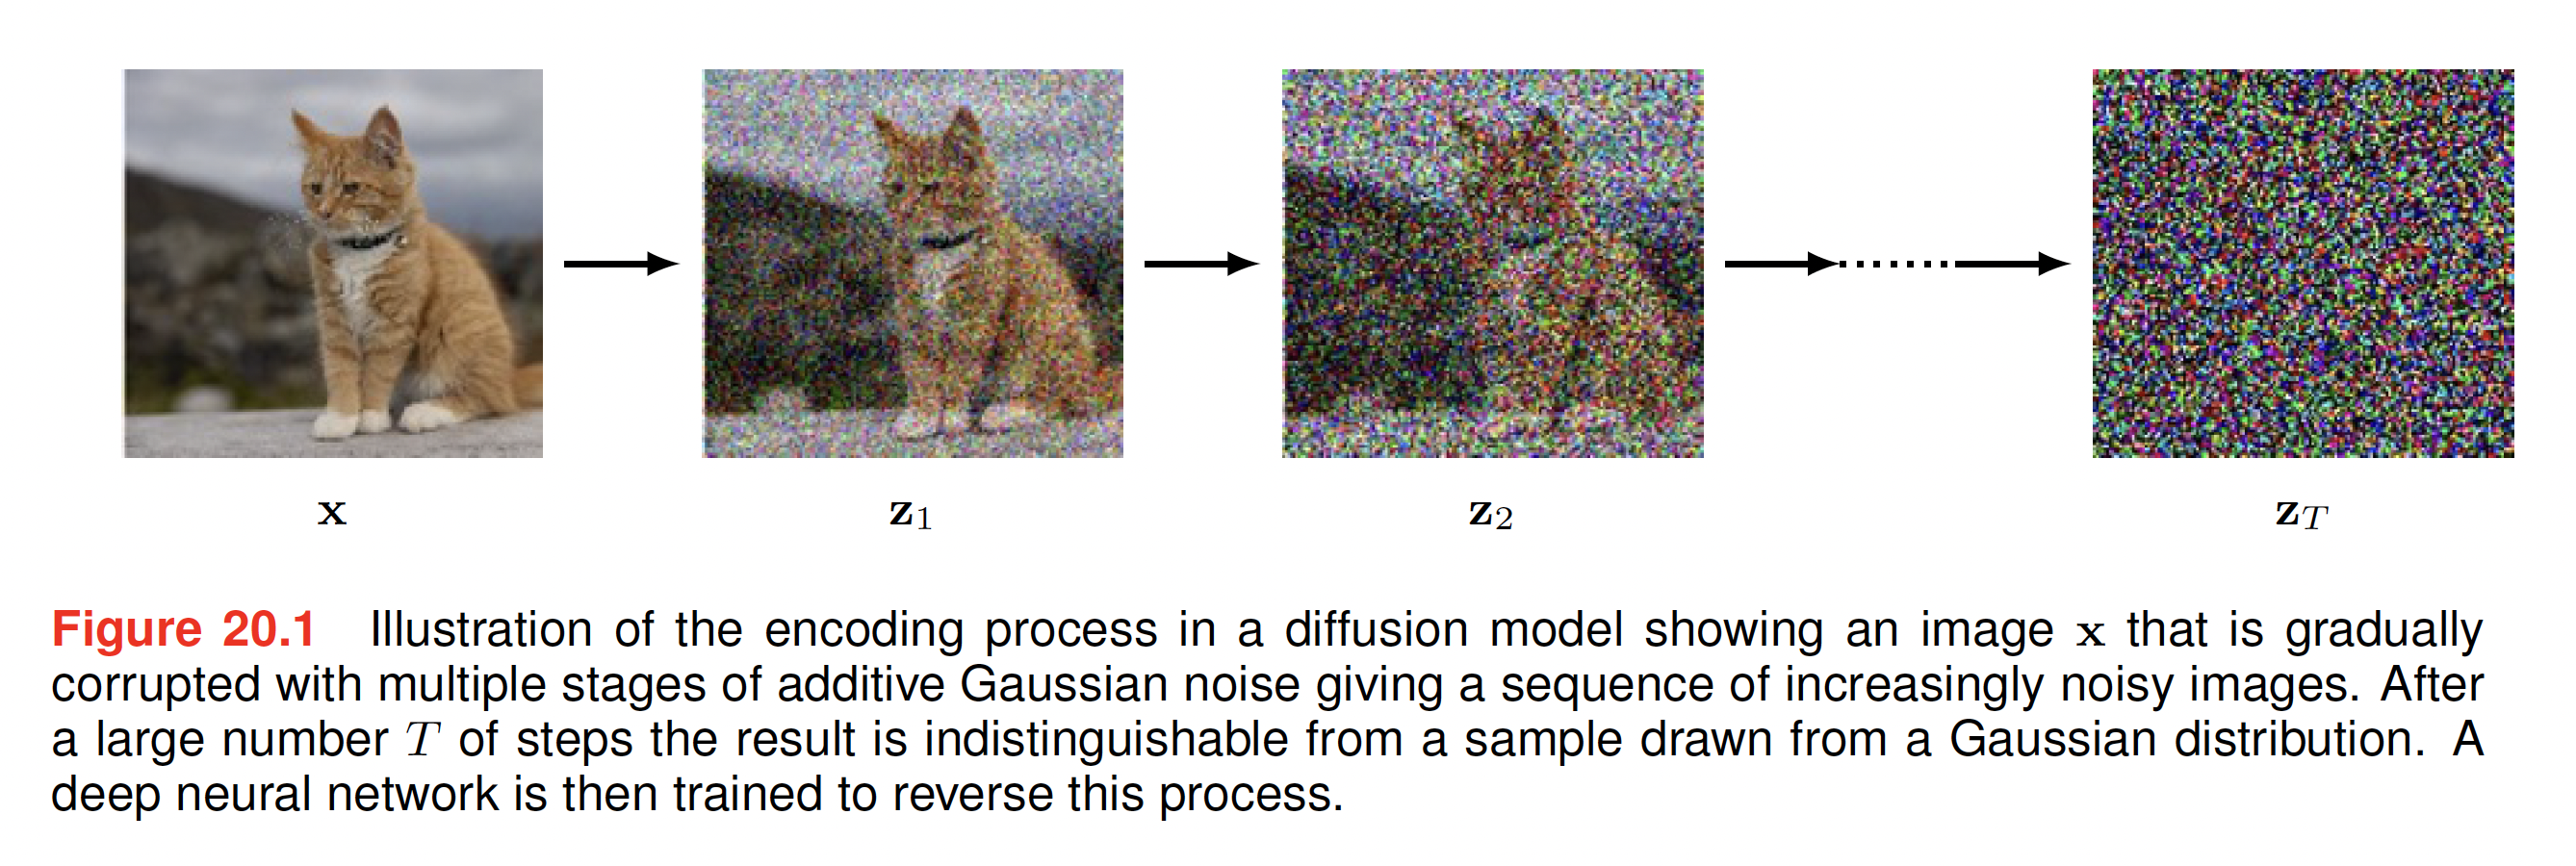
\includegraphics[width=130mm]{cat-diffusion.png}
\end{figure}

\vspace{0.5cm}

Diffusion models are technically not limited to image modeling, but provides a useful motivation.

\end{frame}

%------------------------------------------------
\section{Forward Encoder}
%------------------------------------------------

\begin{frame}{Forward Encoder}

Beginning with an original image $z_0 = x$, we can \alert{corrupt} it with Gaussian noise at each pixel by applying the transformation
\begin{align*}
    z_t = \sqrt{1 - \beta_t} z_{t-1} + \sqrt{\beta_t} \epsilon_t
\end{align*}
for $\epsilon_t \sim \mathcal{N}(\mathbf{0}, \mathbf{I})$. We choose $\beta_t$ such that $z_t$ is closer to $z_{t-1}$ than $\epsilon_t$. We can write the transformation in the form,
\begin{align*}
    q(z_t | z_{t-1}) = \mathcal{N}(\sqrt{1 - \beta_t} z_{t-1}, \beta_t \mathbf{I})
\end{align*}

The values of the variance parameters $\beta_t \in (0, 1)$ are set by hand, such that the variance values increase through the chain according to a prescribed schedule such that $\beta_1 < \beta_2 < \dots < \beta_T$

\end{frame}

%------------------------------------------------

\begin{frame}{Forward Encoder}

\begin{figure}[h!]
\centering
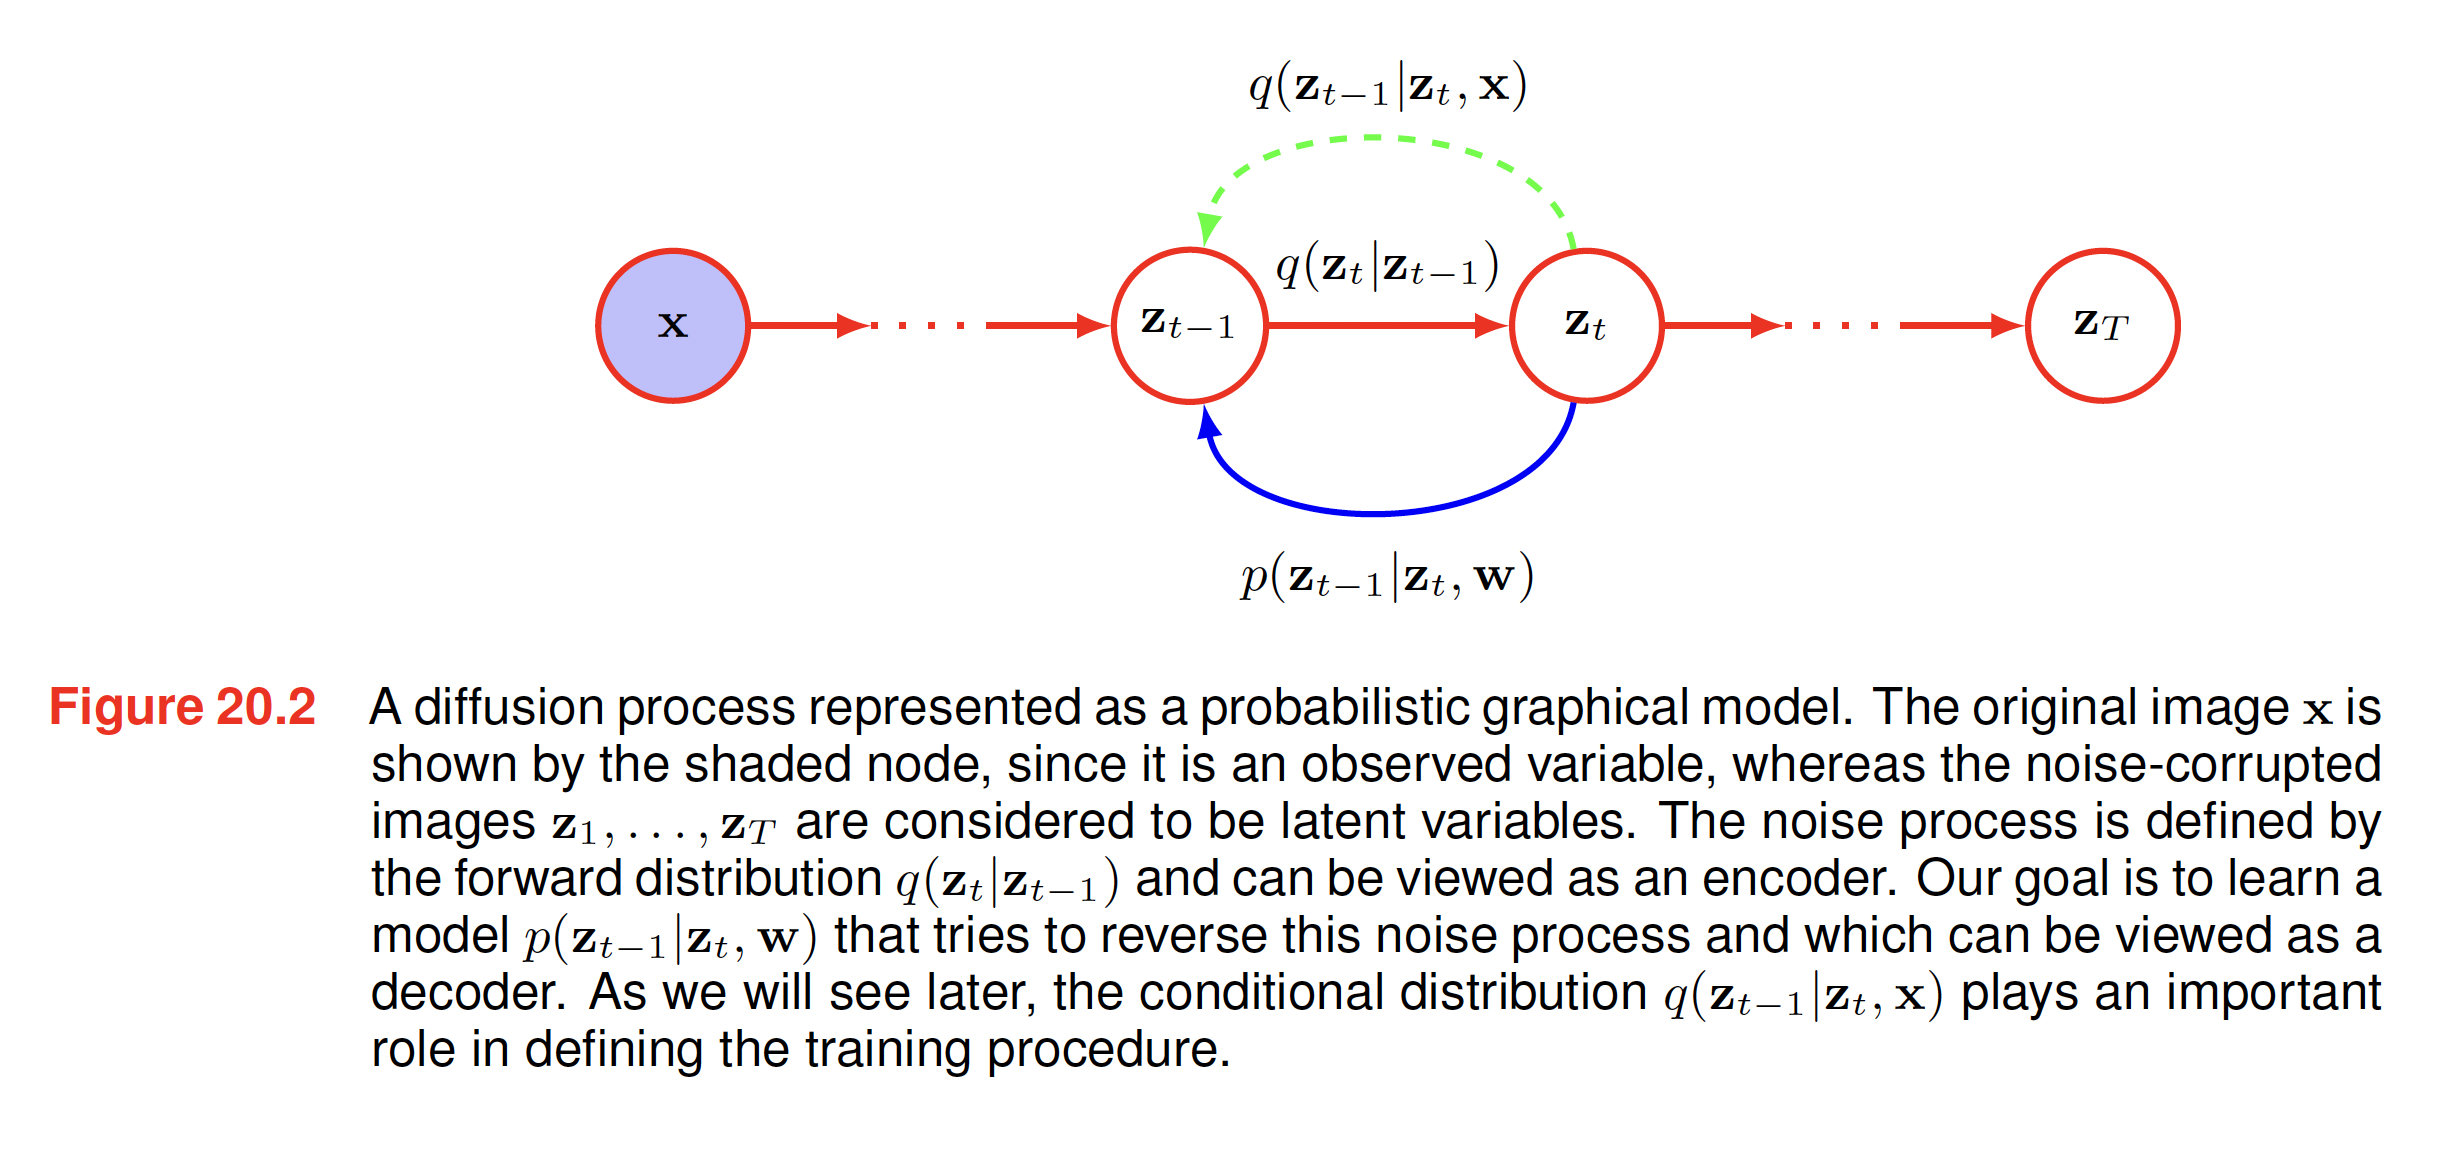
\includegraphics[width=130mm]{forward-markov.png}
\end{figure}
\end{frame}

%------------------------------------------------

\begin{frame}{Forward Encoder}

The joint distribution of the latent variables, conditioned on the observed data vector $x$, is given by
\begin{align*}
    q(z_1, \dots, z_t | x) = q(z_1 | z_0) \prod^{t}_{\tau=1} q(z_\tau | z_{\tau - 1})
\end{align*}

Marginalizing over the intermediate variables $z_1, \dots, z_{t-1}$ gives us the \alert{diffusion kernel}.
\begin{align*}
     q(z_T | z_0) = \mathcal{N}(\sqrt{\alpha_2} z_0, (1 - \alpha_2) \mathbf{I})
\end{align*}
for $\alpha_t = \prod^{t}_{\tau=1}(1-\beta_\tau)$

\end{frame}

%------------------------------------------------

\begin{frame}{Diffusion Kernel}

Let $\alpha_1 = 1 - \beta_1$, we know
\begin{align*}
    z_1 &= \sqrt{\alpha_1} z_0 + \sqrt{1 - \alpha_1}\epsilon_0 \\
    q(z_1 | z_0) &= \mathcal{N}(\sqrt{\alpha_1} z_0, (1-\alpha_1)\mathbf{I})
\end{align*}

Now, for $z_2$,
\begin{align*}
    z_2 &= \sqrt{1-\beta_2} z_1 + \sqrt{\beta_2}\epsilon_1
\end{align*}

Substituting the form we have for $z_1$
\begin{align*}
    z_2 &= \sqrt{1-\beta_2} z_1 + \sqrt{\beta_2}\epsilon_1 \\
    z_2 &= \sqrt{1-\beta_2} (\sqrt{1-\beta_1} z_0 + \sqrt{\beta_1}\epsilon_0) + \sqrt{\beta_2}\epsilon_1 \\
    z_2 &= \sqrt{1-\beta_2}\sqrt{1-\beta_1} z_0 + \sqrt{1-\beta_2}\sqrt{\beta_1}\epsilon_0 + \sqrt{\beta_2}\epsilon_1
\end{align*}

\end{frame}

%------------------------------------------------

\begin{frame}{Diffusion Kernel}

The combined noise terms are in the form of the sum of two Gaussians, which we know to be Gaussian:
\begin{align*}
     Var(\sqrt{1-\beta_2}\sqrt{\beta_1}\epsilon_0 + \sqrt{\beta_2}\epsilon_1) &= \beta_1(1-\beta_2)+\beta_2 \\
     &= 1 - 1 + \beta_1 - \beta_1 \beta_2 + \beta_2 \\
     &= 1 - (1 - \beta_1) - \beta_2 (1 - \beta_1) \\
     &= 1 - (1 - \beta_1)(1-\beta_2) \\
     &= 1 - \alpha_2
\end{align*}

Hence we have shown
\begin{align*}
     q(z_2 | z_0) = \mathcal{N}(\sqrt{\alpha_2} z_0, (1 - \alpha_2) \mathbf{I})
\end{align*}

The rest of the proof proceeds by induction.

\end{frame}

%------------------------------------------------

\begin{frame}{Diffusion Kernel}

This allows efficient stochastic gradient descent using randomly chosen intermediate terms in the Markov chain without having to run the whole chain. We can also write the kernel in the form
\begin{align*}
    z_t = \sqrt{\alpha_t} z_0 + \sqrt{1 - \alpha_t} \epsilon_t
\end{align*}

After many steps $T$ this converges to the stationary distribution
\begin{align*}
    q(z_T | z_0) = \mathcal{N}(\mathbf{0}, \mathbf{I})
\end{align*}
as
\begin{align*}
    \lim_{t \to \infty} \alpha_t = \lim_{t \to \infty} \prod^{t}_{\tau=1}(1-\beta_\tau) = 0
\end{align*}

\end{frame}

%------------------------------------------------
\section{Reverse Decoder}
%------------------------------------------------

\begin{frame}{Reverse Decoder}

The forward encoder model is defined by a sequence of Gaussian
conditional distributions $q(z_t|z_{t-1})$.

\vspace{0.3cm}

However, inverting this directly leads to \alert{a distribution $q(z_{t-1}|z_t)$ that is intractable}, as it would require integrating over all possible values of the starting vector $z_0$.

\vspace{0.3cm}

Recall that the distribution of $z_0$ is the unknown data distribution $p(z_0 = x)$ that we wish to model. 

\vspace{0.3cm}

Instead, we will learn an approximation to the reverse distribution by \alert{using a distribution $p(z_{t-1}|z_t | w)$ governed by a deep neural network}.

\end{frame}

%------------------------------------------------

\begin{frame}{Reverse Decoder}

If $\beta_t << 1$, the distribution $q(z_{t-1}|z_t)$ will be approximately a Gaussian distribution over $z_{t-1}$.

\begin{figure}[h!]
\centering
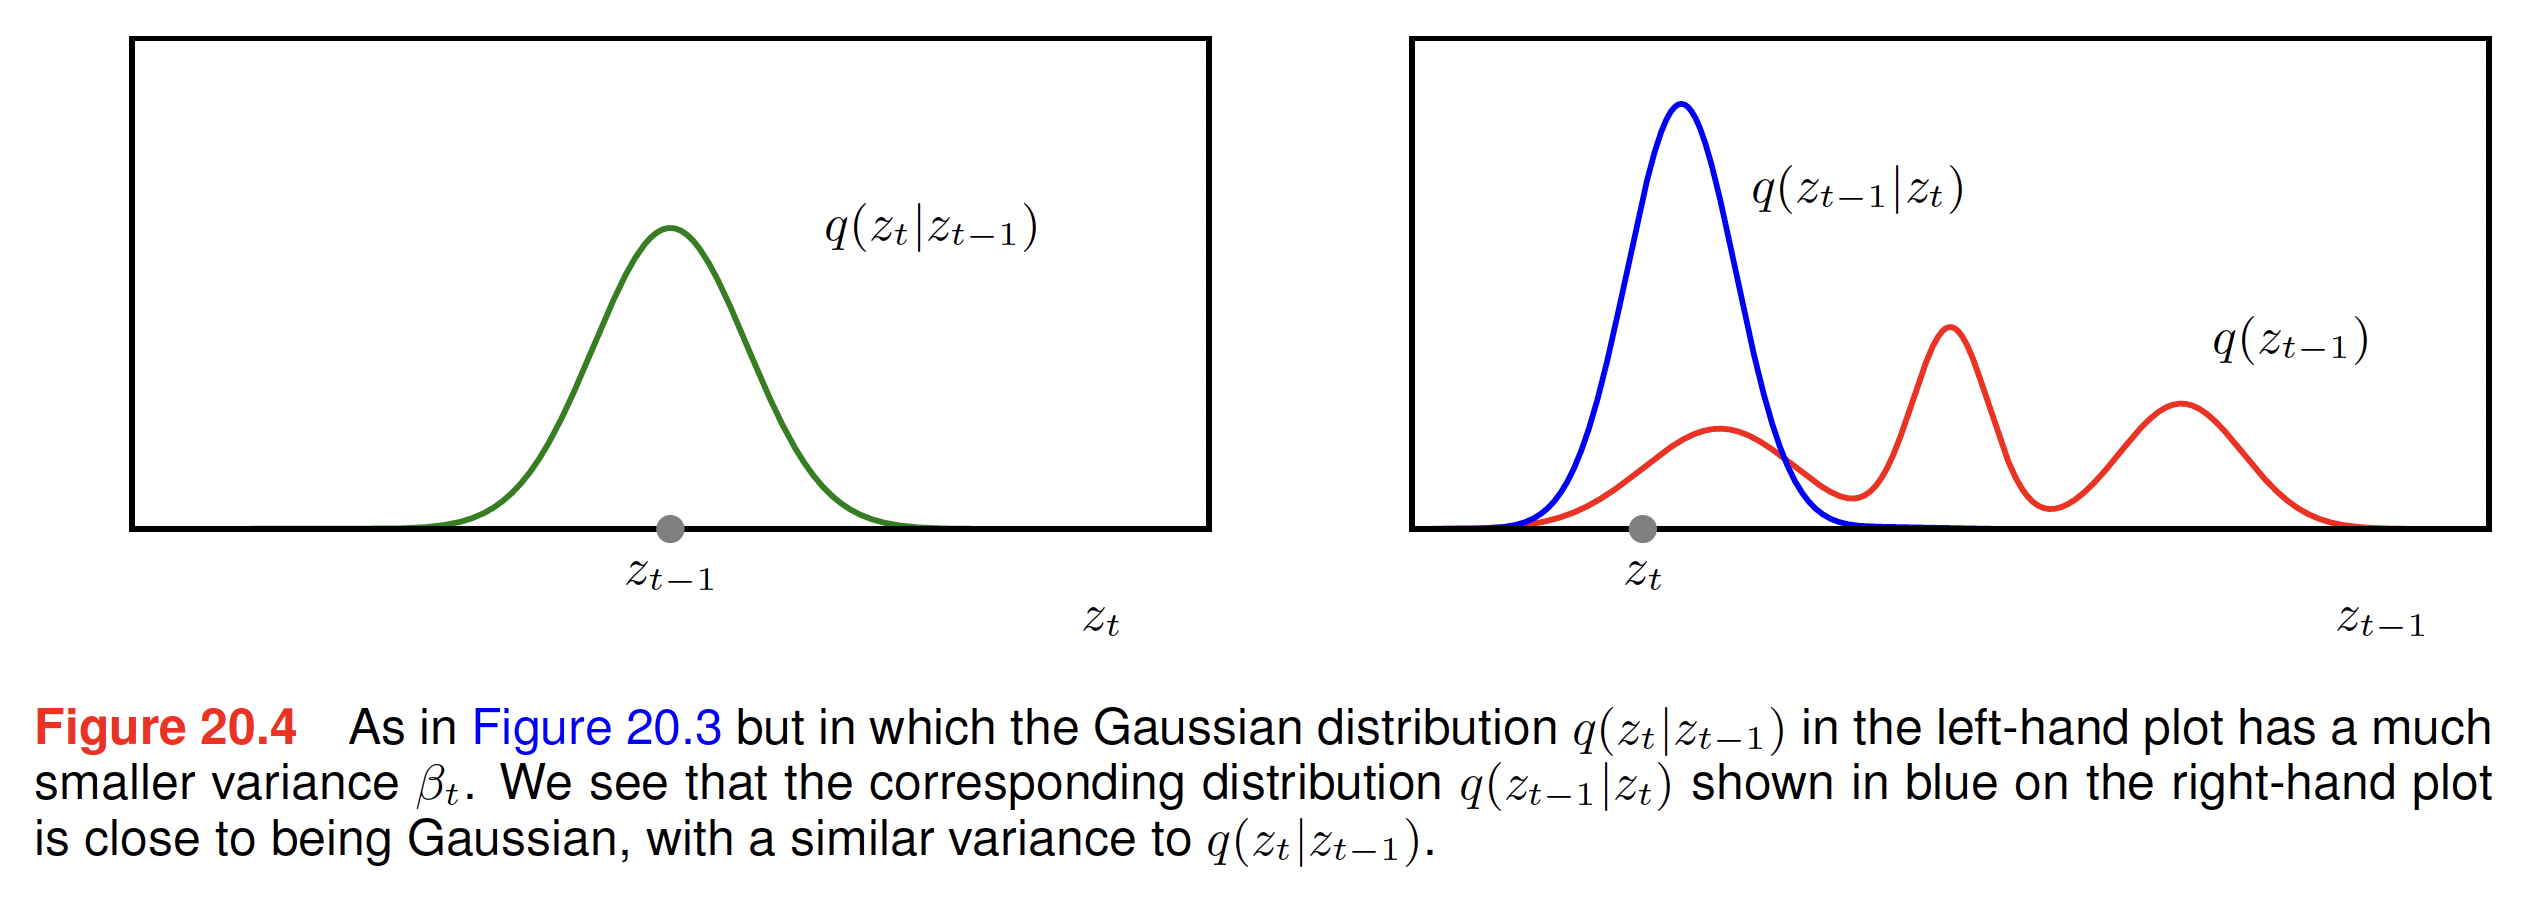
\includegraphics[width=130mm]{gaussian-approx.png}
\end{figure}

\end{frame}

%------------------------------------------------

\begin{frame}{Reverse Decoder}

However, since the variances at each step are small, we \alert{must use a large number of steps}.

\vspace{0.3cm}

This ensure that the distribution over the final latent variable $z_T$ obtained from the forward noising process will still be close to a Gaussian.

\vspace{0.3cm}

This \alert{increases the cost of generating new samples}. In practice, $T$ may be several thousand.

\end{frame}

%------------------------------------------------

\begin{frame}{Reverse Decoder}

The overall reverse denoising process then takes the form of a Markov chain given by
\begin{align*}
p(z_0, z_1, \dots, z_T | w) = p(z_T) \bigg\{ \prod^T_{t=2} p(z_{t-1 | z_t, w}) \bigg\} p(z_0 | z_1, w)
\end{align*}

Here $p(z_T)$ is assumed to be the same as the distribution of $q(z_T)$ and hence is given by $\mathcal{N}(\mathbf{0}, \mathbf{I})$.

\vspace{0.3cm}

Once the model has been trained, we first sample from the simple Gaussian $p(z_T)$ and then again \alert{sequentially from each of the conditional distributions $p(z_{t-1}|z_t, w)$} in turn, finally sampling from $p(x| z_1, w)$ to obtain a sample $z_0 = x$ in the data space.

\end{frame}

%------------------------------------------------

\begin{frame}{Training the Decoder}

The full data log-likelihood involves integrating over all possible trajectories from noise to data point, and hence is intractable.

\vspace{0.3cm}

We can adopt a similar approach to that used with variational autoencoders and maximize a lower bound on the log likelihood, specifically the \alert{evidence lower bound (ELBO)},
\begin{align*}
    \mathcal{L}(w) = \int \ln \bigg\{ \frac{p(x, z, | w)}{q(z)} \bigg\} q(z) = \mathbb{E}\bigg[ \ln \bigg\{ \frac{p(x, z, | w)}{q(z)} \bigg\} \bigg]
\end{align*}

We chose $q(z)$ to be given by the fixed distribution $q(z_1, \dots, z_T |x)$ defined by the Markov chain, and so the only adjustable parameters are those in the model $p(x, z_1, \dots, z_T |w)$ for the reverse Markov chain.

\end{frame}

%------------------------------------------------

\begin{frame}{Training the Decoder}

Rewriting this with the chosen model,
\begin{align*}
    \mathcal{L} &= \mathbb{E}\bigg[ \ln \frac{p(z_T)  \big\{\prod^T_{t=2} p(z_{t-1} | z_t, w) \big\} p(z_0 | z_1, w) }{q(z_1 | z_0) \prod^T_{t=2} q(z_t | z_{t-1}, z_0)} \bigg] \\
    &= \mathbb{E} \bigg[ \ln p(z_T) + \sum^T_{t=2} \ln \frac{p(z_{t-1} | z_t, w)}{q(z_t | z_{t-1}, z_0)} - \ln q(z_1 | z_0) + \ln p(z_0 | z_1, w) \bigg]
\end{align*}

\end{frame}

%------------------------------------------------

\begin{frame}{Training the Decoder}

This expectation is easy to estimate. First, we draw set of $M$ samples of $z_t$. Let $g$ be the complex function inside the expectation. Each $j$th draw $z_t^*$ gives rise to $g^*_j$
\begin{align*}
    g^* = \ln p(z^*_T) + \sum^T_{t=2} \ln \frac{p(z^*_{t-1} | z^*_t, w)}{q(z^*_t | z^*_{t-1}, z^*_0)} - \ln q(z^*_1 | z_0) + \ln p(z^*_0 | z^*_1, w)
\end{align*}

The expectation $\mathbb{E}[g]$ then just becomes
\begin{align*}
    \mathbb{E}[g] \approx \sum^M_{j=1} g^*_j
\end{align*}

\end{frame}

%------------------------------------------------

\begin{frame}{Training the Decoder}

\begin{algorithmic}
    \Require Training data $\mathcal{D} = \{\mathbf{x}_n\}$, Noise schedule $\{\beta_1, \dots, \beta_T\}$
    \Statex

    \For{$t \in \{1, \dots, T\}$}
        \State $\alpha_t \gets \prod_{\tau=1}^{t} (1 - \beta_\tau)$ \Comment{Calculate alphas from betas}
    \EndFor

    \Statex

    \Repeat
        \State $\mathbf{x} \sim \mathcal{D}$ \Comment{Sample a data point}
        \State $t \sim \text{Uniform}(\{1, \dots, T\})$ \Comment{Sample a point along the Markov chain}
        \State $\boldsymbol{\epsilon} \sim \mathcal{N}(\mathbf{0}, \mathbf{I})$ \Comment{Sample a noise vector}
        \State $\mathbf{z}_t \gets \sqrt{\alpha_t}\mathbf{x} + \sqrt{1-\alpha_t}\boldsymbol{\epsilon}$ \Comment{Evaluate noisy latent variable}
        \State $\mathcal{L}(\mathbf{w}) \gets \|\modelg(\mathbf{z}_t, \mathbf{w}, t) - \boldsymbol{\epsilon}\|^2$ \Comment{Compute loss term}
        \State Take optimizer step on $\nabla_{\mathbf{w}}\mathcal{L}(\mathbf{w})$
    \Until{converged}
\end{algorithmic}

\end{frame}

%------------------------------------------------

\begin{frame}[fragile]{Training the Decoder}
\scriptsize
\begin{lstlisting}
def q_sample(self, x_start, t, noise=None):
    """Forward process: add noise to an image."""
    if noise is None:
        noise = torch.randn_like(x_start)

    sqrt_alphas_cumprod_t = self.sqrt_alphas_cumprod[t].view(-1, 1, 1, 1)
    sqrt_one_minus_alphas_cumprod_t = self.sqrt_one_minus_alphas_cumprod[t].view(-1, 1, 1, 1)
    
    return sqrt_alphas_cumprod_t * x_start + sqrt_one_minus_alphas_cumprod_t * noise
\end{lstlisting}

\end{frame}

%------------------------------------------------

\begin{frame}{Sampling from the Decoder}

\begin{algorithmic}[1]
    \Require Trained denoising network $\modelg(\mathbf{z}, \mathbf{w}, t)$, Noise schedule $\{\beta_1, \dots, \beta_T\}$
    \State $\mathbf{z}_T \sim \mathcal{N}(\mathbf{0}, \mathbf{I})$ \Comment{Sample from final latent space}

    \Statex

    \For{$t = T, \dots, 2$}
        \State $\alpha_t \gets \prod_{\tau=1}^{t} (1 - \beta_\tau)$ \Comment{Calculate alpha}
        \Statex \Comment{Evaluate network output}
        \State $\boldsymbol{\mu}(\mathbf{z}_t, \mathbf{w}, t) \gets \frac{1}{\sqrt{1-\beta_t}}\left\{\mathbf{z}_t - \frac{\beta_t}{\sqrt{1-\alpha_t}}\modelg(\mathbf{z}_t, \mathbf{w}, t)\right\}$
        \State $\boldsymbol{\epsilon} \sim \mathcal{N}(\mathbf{0}, \mathbf{I})$ \Comment{Sample a noise vector}
        \State $\mathbf{z}_{t-1} \gets \boldsymbol{\mu}(\mathbf{z}_t, \mathbf{w}, t) + \sqrt{\beta_t}\boldsymbol{\epsilon}$ \Comment{Add scaled noise}
    \EndFor

    \Statex

    \State $\mathbf{x} \gets \frac{1}{\sqrt{1-\beta_1}}\left\{\mathbf{z}_1 - \frac{\beta_1}{\sqrt{1-\alpha_1}}\modelg(\mathbf{z}_1, \mathbf{w}, 1)\right\}$ \Comment{Final denoising step}
    
\end{algorithmic}

\end{frame}

%------------------------------------------------

\begin{frame}[fragile]{Sampling from the Decoder}
\scriptsize
\begin{lstlisting}
@torch.no_grad()
def sample(model, diffusion, n_images, img_size, channels=3, device="cpu"):
    """Samples new images from the diffusion model."""
    model.eval()
    
    img = torch.randn((n_images, channels, img_size, img_size), device=device)
    
    images = []
    for t in tqdm(reversed(range(0, diffusion.timesteps)), desc="Sampling", 
                    total=diffusion.timesteps):
        t_tensor = torch.full((n_images,), t, device=device, dtype=torch.long)
        predicted_noise = model(img, t_tensor)

        alpha_t = diffusion.alphas[t]
        alpha_t_cumprod = diffusion.alphas_cumprod[t]
        beta_t = diffusion.betas[t]

        """More code below"""
\end{lstlisting}

\end{frame}

%------------------------------------------------

\begin{frame}[fragile]{Sampling from the Decoder}
\scriptsize
\begin{lstlisting}
        """Continued from previous slide"""
        term1 = 1 / torch.sqrt(alpha_t)
        term2 = (beta_t / torch.sqrt(1 - alpha_t_cumprod)) * predicted_noise
        img = term1 * (img - term2)
        
        if t > 0:
            noise = torch.randn_like(img)
            img += torch.sqrt(beta_t) * noise
            
        if t % 50 == 0:
            images.append(img.cpu().numpy())
            
    return img.cpu(), images
\end{lstlisting}

\end{frame}

%------------------------------------------------

\begin{frame}{Sampling from the Decoder}

\begin{columns}[T]
    \begin{column}{0.05\textwidth}
        
    \end{column}
    \begin{column}{0.25\textwidth}
        \vspace{2em}
        
        \scriptsize
        Example of training a U-Net to sample images of a square.

        \vspace{1em}
        
        The full code is available on my github: \href{https://github.com/dominicdayta/diffuser}{@dominicdayta/diffuser}
        \normalsize
    \end{column}
    \begin{column}{0.7\textwidth}
        \centering
        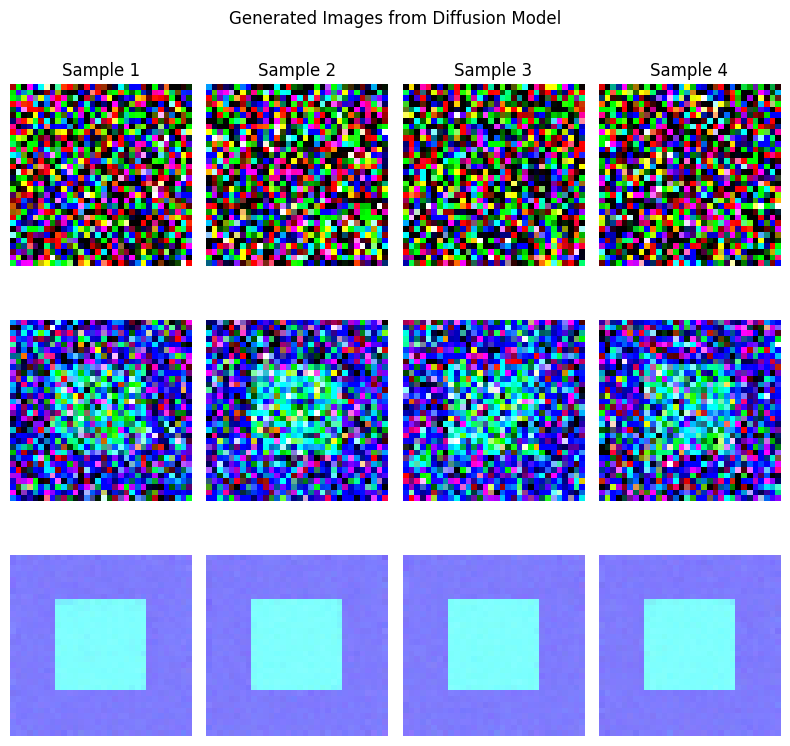
\includegraphics[width=65mm]{squares.png}        
    \end{column}
\end{columns}

\end{frame}

%------------------------------------------------
\section{Score Matching}
%------------------------------------------------

\begin{frame}{Score Matching}

\begin{columns}[T]
    \begin{column}{0.6\textwidth}
        \begin{itemize}
            \item At any step $t$, the noisy data distribution is $q(\mathbf{z}_t)$.
            \item The \alert{score function} is defined as the gradient of the log-probability of this distribution with respect to the data:
            $$ \nabla_{\mathbf{z}_t} \log q(\mathbf{z}_t) $$
            \item he score is a vector field that points in the direction where the data density is increasing most rapidly.
            \item If we could learn this score function, we could \alert{use it to guide a reverse process}, starting from random noise and moving towards regions of high data probability to generate a sample.
        \end{itemize}
    \end{column}
    \begin{column}{0.4\textwidth}
        \centering
        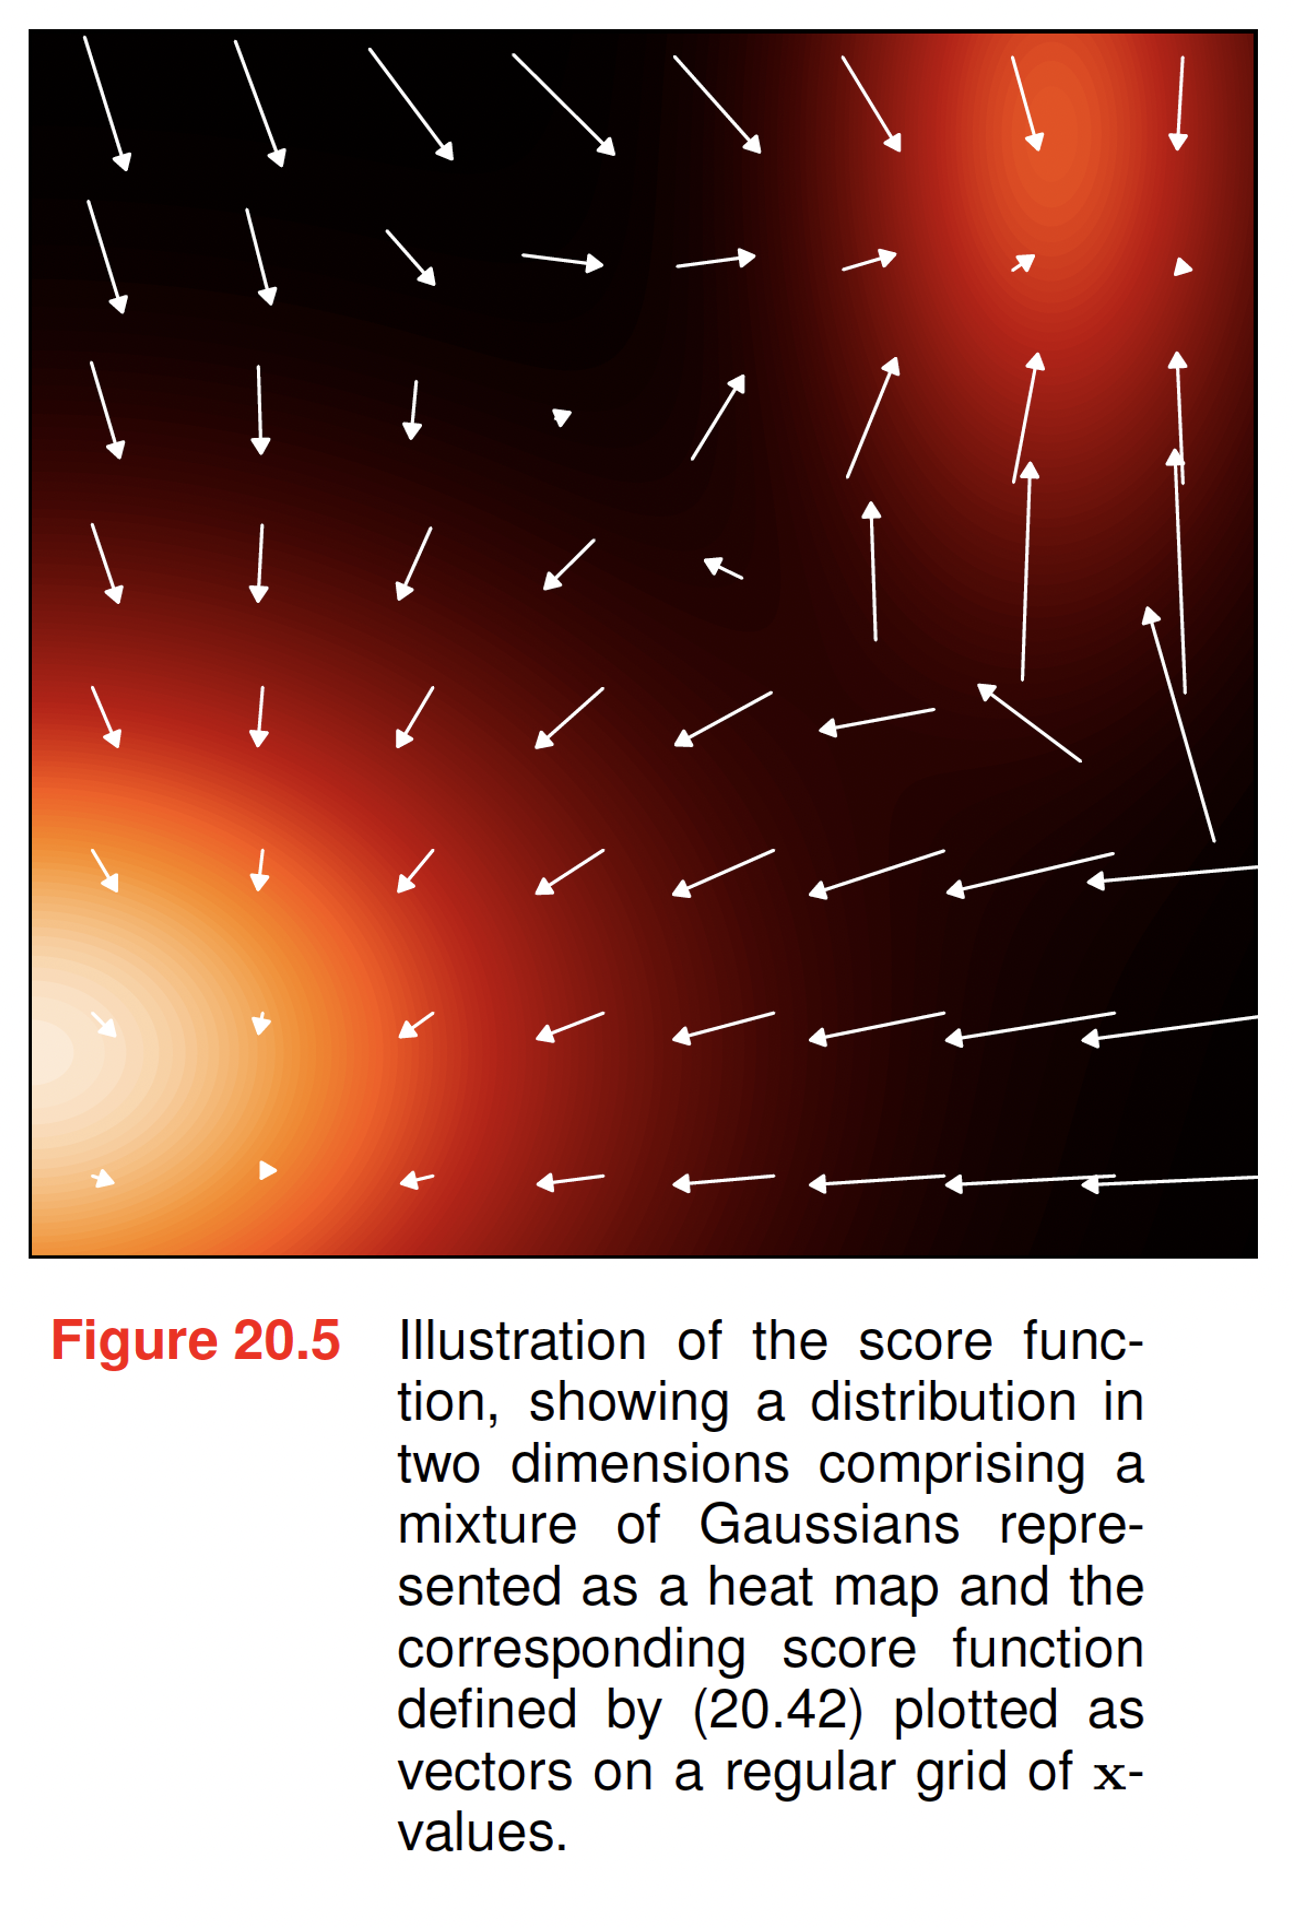
\includegraphics[width=0.7\textwidth]{score-matching.png}
    \end{column}
\end{columns}

\end{frame}

%------------------------------------------------

\begin{frame}{Score Matching}

The core idea of score matching is to train a neural network, our \alert{score model} $\mathbf{s}(\mathbf{z}_t, \mathbf{w}, t)$, to approximate the true (but unknown) score function.

\vspace{1em}

We can define a loss function by \alert{minimizing the expected squared distance} between our model's prediction and the true score:
\begin{equation}
    \mathcal{L}_{SM}(\mathbf{w}) = \mathbb{E}_{q(\mathbf{z}_t)} \left[ \| \mathbf{s}(\mathbf{z}_t, \mathbf{w}, t) - \nabla_{\mathbf{z}_t} \log q(\mathbf{z}_t) \|^2 \right]
\end{equation}

\vspace{1em}

\begin{itemize}
    \item This objective directly trains our model to learn the gradient field of the data distribution.
    \item However, this formulation is \alert{still intractable} because the target $\nabla_{\mathbf{z}_t} \log q(\mathbf{z}_t)$ depends on the unknown distribution $q(\mathbf{z}_t)$.
\end{itemize}

\end{frame}

%------------------------------------------------

\begin{frame}{Score Matching}

The solution is \alert{Denoising Score Matching}.

\vspace{1em}

The score of the conditional distribution $q(\mathbf{z}_t|\mathbf{x})$, which we can define, is directly related to the noise $\boldsymbol{\epsilon}$ that was added:

\begin{align*}
    \nabla_{\mathbf{z}_t} \log q(\mathbf{z}_t | \mathbf{x}) = -\frac{\mathbf{z}_t - \sqrt{\alpha_t}\mathbf{x}}{1-\alpha_t} = -\frac{\boldsymbol{\epsilon}}{\sqrt{1-\alpha_t}}
\end{align*}

\end{frame}

%------------------------------------------------

\begin{frame}{Score Matching}

It can be shown that minimizing the denoising objective is equivalent to minimizing the score matching objective.

\vspace{0.5em}

Let our score model be defined by our noise-prediction network $\mathbf{g}(\mathbf{z}_t, \mathbf{w}, t)$:
    $$ \mathbf{s}(\mathbf{z}_t, \mathbf{w}, t) := -\frac{\mathbf{g}(\mathbf{z}_t, \mathbf{w}, t)}{\sqrt{1-\alpha_t}} $$

The \alert{denoising loss} from Algorithm 20.1 is:
    $$ \mathcal{L}(\mathbf{w}) = \mathbb{E}_{t, \mathbf{x}, \boldsymbol{\epsilon}} \left[ \| \mathbf{g}(\mathbf{z}_t, \mathbf{w}, t) - \boldsymbol{\epsilon} \|^2 \right] $$

Training a network $\mathbf{g}$ to predict the noise $\boldsymbol{\epsilon}$ is mathematically equivalent to training a network $\mathbf{s}$ to predict the score $\nabla_{\mathbf{z}_t} \log q(\mathbf{z}_t)$.

\end{frame}

%------------------------------------------------
\section{Guided Diffusion}
%------------------------------------------------

\begin{frame}{Guided Diffusion}

The diffusion models we have seen so far are \alert{unconditional generators}: they learn the entire distribution $p(\mathbf{x})$. In consequence, they can generate high-quality samples that look like the training data.

\vspace{1em}

However, we have \alert{no control over the output}. We cannot ask the model to generate an image of a specific class or with specific attributes.

\vspace{1em}

Instead, we want to steer the generation process to sample from a \alert{conditional distribution} $p(\mathbf{x}|\mathbf{y})$, where $\mathbf{y}$ is some conditioning information, such as:
\begin{itemize}
    \item A class label (e.g., "cat", "dog", "car").
    \item A text description (e.g., "a photo of an astronaut riding a horse").
    \item Another image (for image-to-image translation).
\end{itemize}

\end{frame}

%------------------------------------------------

\begin{frame}{Guided Diffusion}

The core idea is to \alert{guide the reverse diffusion process} towards a desired class $\mathbf{y}$.

\vspace{0.5em}

\begin{enumerate}
    \item We start with our standard unconditional diffusion model that predicts the score $\nabla_{\mathbf{z}_t} \log q(\mathbf{z}_t)$.
    \item We separately train a classifier $p(\mathbf{y}|\mathbf{z}_t)$ that learns to predict the class label $\mathbf{y}$ from a noisy image $\mathbf{z}_t$.
\end{enumerate}

\end{frame}

%------------------------------------------------

\begin{frame}{Guided Diffusion}

Using Bayes' theorem, the score of the desired \textit{conditional} distribution is:
\begin{align*}
    \underbrace{\nabla_{\mathbf{z}_t} \log q(\mathbf{z}_t|\mathbf{y})}_\text{Guided Score} = \underbrace{\nabla_{\mathbf{z}_t} \log q(\mathbf{z}_t)}_\text{Unconditional Score} + \underbrace{\nabla_{\mathbf{z}_t} \log p(\mathbf{y}|\mathbf{z}_t)}_\text{Classifier Gradient}
\end{align*}

At each step $t$, we modify the mean of the reverse step. We nudge it in the direction of the classifier's gradient. A guidance scale $s$ controls the strength of this effect.

\vspace{1em}

This approach requires training and maintaining a separate classifier model on noisy images, which can be complex and unstable.

\end{frame}

%------------------------------------------------

\begin{frame}{Guided Diffusion}

A more elegant and powerful solution is to make the diffusion model itself handle the conditioning.
\begin{itemize}
    \item The U-Net model is now conditioned on the class label $\mathbf{y}$: $\mathbf{g}(\mathbf{z}_t, \mathbf{w}, t, \mathbf{y})$.
    \item During training, we randomly replace the true label $\mathbf{y}$ with a null label $\varnothing$ (e.g., 10-20\% of the time).
    \item This forces the \alert{same model} to learn both the \textit{conditional} prediction $\mathbf{g}(\dots, \mathbf{y})$ and the \textit{unconditional} prediction $\mathbf{g}(\dots, \varnothing)$.
\end{itemize}

\end{frame}

%------------------------------------------------

\begin{frame}{Guided Diffusion}

At each sampling step, we \alert{compute both predictions and extrapolate} from the unconditional towards the conditional estimate:
\begin{align*}
    \hat{\boldsymbol{\epsilon}} = \underbrace{\boldsymbol{\epsilon}_\theta(\mathbf{z}_t, \varnothing)}_\text{Unconditional} + s \cdot \Big( \underbrace{\boldsymbol{\epsilon}_\theta(\mathbf{z}_t, \mathbf{y})}_\text{Conditional} - \underbrace{\boldsymbol{\epsilon}_\theta(\mathbf{z}_t, \varnothing)}_\text{Unconditional} \Big)
\end{align*}

The term in parentheses is the "guidance direction".

\vspace{1em}

The guidance scale $s > 1$ pushes the prediction further in this direction, improving sample quality and adherence to the condition $\mathbf{y}$.

\vspace{1em}

Classifier-free guidance is simpler to implement, more stable to train, and generally produces higher-quality results. It is the standard for modern diffusion models.
\end{frame}

%------------------------------------------------

\begin{frame}{Guided Diffusion}

\begin{figure}[h!]
\centering
\includegraphics[width=120mm]{panda.png}
\end{figure}

\end{frame}


%------------------------------------------------

\end{document}